\chapter{Symmetric two team Markov game}\label{ch:2teams}
\begin{chapter_outline}

This chapter presents how to combine cooperative and competitive to train two teams to compete.
Section \ref{sec:ch7_intro} introduces the motivations behind this study.
Following this, we define the two-team Markov game in Section \ref{sec:ch7_2teammarkov} and the adaptation of SMAC to this mixed cooperative-competitive framework in Section \ref{sec:ch7_competsmac}.
Section \ref{sec:ch7_learningscenar} describes the learning scenarios used to train and how to evaluate teams, followed by the experimental setup in Section \ref{sec:ch7_experiments}.
The corresponding results are presented in Section \ref{sec:ch7_results}, and we conclude this chapter with discussions in Section \ref{sec:ch7_conclu}.

This chapter is an adapted version of the publication~\citep{leroy2022twoteam} \textit{Value-based CTDE methods in symmetric two-team Markov game: from cooperation to team competition}, P. Leroy, J. Pisane, and D. Ernst. Deep Reinforcement Learning Workshop NeurIPS, 2022

\end{chapter_outline}

\section{Introduction} \label{sec:ch7_intro}

Many applications exist where two teams of multiple agents compete, such as in games (Pommerman \citep{resnick2018pommerman}) or in robotics (RoboCup \citep{kitano1997robocup}).
In certain use cases, agents are not fully aware of the entire environment, such as in Cyber-Physical Production Systems \citep{phan2020learning}, Hide and Seek \citep{baker2019emergent} or Capture the Flag \citep{jaderberg2019human}.
In this chapter, we combine the cooperative methods from Part \ref{part:coop} with the competitive ones defined in Chapter \ref{ch:competition} to train teams to compete in a mixed cooperative-competitive POSG.
The setting is defined as a symmetric two-team Markov game where two teams of the same agents compete.
The goal is to identify how to train a team to be resilient to different adversarial strategies.

Specifically, we study the difference between three learning scenarios: learning against a stationary team policy, against a single evolving team strategy (self-play), and against multiple evolving team strategies within a population of learning teams.
To evaluate the performance of each learning scenario, we created a new competitive environment suite by modifying SMAC, initially designed for cooperation and defined in Section \ref{sec:ch3_smac}.
We chose symmetrical competition to ensure fair and balanced competition, as well as the possibility of controlling either team with the same agents.
In two different SMAC environments, teams are trained with the three value-based CTDE methods, QMIX, MAVEN, and QVMix, each with three learning scenarios.
These methods are defined in Section \ref{sec:ch3_value}.
We then analyse how they perform when faced with multiple opposing strategies by forming test populations of trained teams.
Our results suggest that when competing against several possible strategies, teams trained in a population achieve the best performance, but a selection process is required to select the best team.
We reached this conclusion irrespective of whether or not the stationary strategy was better than all trained teams.

\section{Two-team Markov game}\label{sec:ch7_2teammarkov}

Our framework is a special case of a POSG defined in Chapter \ref{ch:background} with a reward function that provides two rewards, one per team.
Specifically, we are in a symmetric, mixed cooperative-competitive, partially observable two-team Markov game defined by a tuple $[\mathcal{S}, \mathcal{Z}, \mathcal{U}, n, O, R, P, \gamma, T, p]$.
The components of this tuple are similar to the ones defined in the stochastic game in Section \ref{sec:ch2_stochastic_Game} or in the Dec-PODMP in Section \ref{sec:ch3_decpomdp}, and we hereafter define only the different ones.
The main one is that $2n$ agents learn in this framework, divided into two teams of $n$ agents.
Let $\mathcal{I}=\{1,..,n\}$ and $\mathcal{J}=\{1,-1\}$, the $i^{th}$ agent of the $j^{th}$ team is denoted by $a_{i, j}$ with $i \in \mathcal{I}$ and $ j \in \mathcal{J}$.
Since we assume team symmetry, agents $a_{i, 1}$ and $a_{i, -1}$ share the same action space $\forall i$, leading to only one team joint action space $\mathcal{U}=\bigtimes_{i\in \mathcal{I}} \mathcal{U}_{{a_{i, 1}}} = \bigtimes_{i\in \mathcal{I}} 
\mathcal{U}_{{a_{i, -1}}}$.
This leads the transition function to be defined by $P: \mathcal{S} \times \mathcal{U}^2 \rightarrow \Delta(\mathcal{S})$.
The symmetry also induces that agents $a_{i, 1}$ and $a_{i, -1}$ have a similar uncertainty about the state $\forall i$.
Still, obviously, the observation function $O: \mathcal{S} \times I \times J \rightarrow \Delta(\mathcal{Z})$ maps a state to different observations for the same $i$.
Common team rewards $\{r_t^1, r_t^{-1}\} = R(s_{t+1}, s_t, \mathbf{u_t}): \mathcal{S}^2 \times \mathcal{U}^2 \rightarrow \mathbb{R}^2$ are assigned to agents after each timestep.
The goal of each agent $a_{i, j}$ to maximise its expected return $\mathbb{E}_{\mathbf{\pi}, p, P}\left[ \sum_{t=0}^{T-1} \gamma^t r^{j}_t \right]$ where the joint policy $\pi \in \mathcal{U}^2$.
Finally, the symmetry allows the policy of agent $a_{i, 1}$ to select actions of the agent $a_{i, -1}$ $\forall i$.

If one team is constrained to have a stationary policy, the other team would then be the only one learning, and the two-team Markov game can be considered a Dec-POMDP.
In our experiments, teams are trained with value-based CTDE methods designed for Dec-POMDP.
We chose QMIX because of its popularity, MAVEN because of its improved exploration capability, which outperforms QMIX in complex scenarios, and QVMix because it has proven competitive with these two as illustrated in Chapter \ref{ch:qvmix}.

\section{Competitive StarCraft Multi-agent challenge} \label{sec:ch7_competsmac}

To perform our experiments, we created a new environment by modifying SMAC to create a competitive environment. 
We adapted\footnote{\label{foot_note_code}\url{github.com/PaLeroy/competSmac} - \url{github.com/PaLeroy/competPymarl}} both SMAC and the associated learning framework PyMARL \citep{samvelyan2019starcraft}.
It is now possible to control both opposing teams in SMAC and train them simultaneously.
In competitive SMAC, the goal remains unchanged, and it is to defeat the opposing team by inflicting sufficient damage to reduce the hit points of all opponents to zero.
However, unlike in Chapter \ref{ch:qvmix} experiments, the winning team is the one that ends up with the highest sum of remaining hit points at the end.
It is a draw if both teams end up with the same total of hit points.
We have chosen the $3m$ and $3s5z$ maps for our experiments but increased the time horizon.
In the $3m$ map, two teams of three marines compete for a maximum of $100$ timesteps.
In the $3s5z$ map, two teams of three stalkers and five zealots compete for a maximum of $150$ timesteps.
Additionaly, agents observe their relative position with respect to the centre of the map.
More details about these two maps and SMAC can be found in Section \ref{sec:ch3_smac}.

\section{Learning scenarios and performances criteria} \label{sec:ch7_learningscenar}
We aim to train a team to be resilient to different adversarial strategies.
We test three different learning scenarios differentiated by the diversity of opponents' strategies encountered during training.
The trained teams can act as any of the two teams in our environments thanks to the environment symmetry.
In the first learning scenario, the team is trained against a stationary strategy, which we refer to as a heuristic.
As explained in Section \ref{sec:ch7_2teammarkov}, such configuration is a Dec-POMDP and is the framework for which CTDE methods are designed.
The second learning scenario is self-play, in which the team is trained by playing against itself, thus facing a strategy that continuously improves at the same learning speed.
In the third scenario, a population composed of several teams is trained with the same method.
Teams either play against themselves or against other learning teams.
Self-play is the special case of a training population composed of a single team.
In this study, the size of the training population is fixed to five to reduce computational complexity.

After training, we evaluate teams with the Elo rating system \citep{elo1978rating}.
The purpose of the Elo rating system is to assign each population player with a rating $R$ to rank them.
From these ratings, one can compute the probability that a player will win when facing another.
Let $R_A$ and $R_B$ be the ELO scores of players A and B, respectively.
The probability that player A wins over player B is $E_A=\frac{10^{R_A/400}}{10^{R_A/400} + 10^{R_B/400}}$ and the probability that B wins over A is $E_B=\frac{10^{R_B/400}}{10^{R_A/400} + 10^{R_B/400}}$.
One can see that $E_A + E_B = 1$.
The number $400$ can be considered as a parameter.
It determines that if player A's Elo score is 400 points above that of B, it has a ten-times greater chance of defeating B.
In order to update player $A$'s rating after a game, we take into account its score $S_A$, which is equal to $1$ for a win, $0$ for a loss, and $0.5$ for a draw.
The updated score is $R'_A = R_A + cst * (S_A - E_A)$ where $cst$ is a constant that defines the maximum possible update of the Elo score.
Typically, $cst$ is $32$ but for our experiments, we set it to $10$ to decrease the amplitude of oscillations in the Elo score during tests.

We form test populations to compute Elo scores in different configurations.
To evaluate only the learning scenarios, we form one test population for each CTDE method with teams trained with all learning scenarios.
To evaluate the heuristic's performance, we add it to the previously defined test populations to form new ones.
To find the best learning scenario/training method pair, we group all trained teams in two test populations, with and without the heuristic.
To evaluate training efficiency and heuristic performances, each trained team is tested along training against the heuristic and against teams trained with other learning scenarios but using the same CTDE method.

\section{Experiments} \label{sec:ch7_experiments}

For our experiments, teams were trained with three learning scenarios and with three CTDE methods, in two different environments.
We conducted the same experimental process for both environments.
Each method's learning scenario was executed ten times and stopped after each team had exploited $10^7$ samples.
For each method, this resulted in ten teams trained against the heuristic requiring $10^7$ environment timesteps, ten teams trained in self-play requiring $5\times10^6$ environment timesteps and ten training populations of five teams leading to $50$ teams trained within populations requiring at least $5\times10^7$ environment timesteps.
Therefore, $210$ teams of nine types were trained in both environments.

To train teams against the heuristic, it was ensured that they play the same number of episodes, acting as team $j=1$ and team $j=-1$.
Concerning training within a population, each team had an equal chance of playing as either team and an equal chance of playing against any team in the population, including itself.
Network architectures and parameters are identical for all learning scenarios and methods to ensure fair comparison.
The default configurations provided by their different authors \citep{Rashid2018,Mahajan2019MAVEN:Exploration,leroy2020qvmix} determined learning parameters.
However, the epsilon anneal time is set to $2$ million instead of $0.5$ million and the networks are updated every eight episodes in $3m$ and every episode in $3s5z$.
As in the literature, individual networks of each team share the same parameters to improve learning speed. 
Appendix \ref{app:train_param} provides more details about the training parameters, and we present training times in Appendix \ref{app:train_time}.

The heuristic policy is based on two rules.
It moves toward the starting point of the opponent's team until it reaches the opposite side of the map and stops.
If enemies are within shooting range, the agent attacks the nearest one.
This heuristic slightly differs from StarCraft's built-in AI originally used to train teams to cooperate in SMAC.
The built-in AI also moves toward the other side but selects targets based on a priority score.
It will choose to attack the closest unit with the highest priority, which will remain the target until its priority drops or it can no longer be attacked.
A unit's priority score is based on its type and current action.
For example, if two of the same units attack and the targeted unit stops attacking, its priority score will drop, and the built-in AI will select the other unit to attack.
This is the main difference with our heuristic which will attack the nearest unit regardless of its action and priority.
Results show that our heuristic is harder to beat than the one provided in SMAC.
Finally, while both maps are denoted as easy in \citep{samvelyan2019starcraft}, the task of learning everything from scratch is not.
When learning against the heuristic, teams do not need to learn how to find their opponents because they automatically move towards them.
When they learn through self-play or within a population, they first need to learn where to find opponents before they can face them.
This increased complexity compared to the original SMAC led us to choose these maps, motivated by a compromise between computational complexity and learning complexity.

As described in Section \ref{sec:ch7_learningscenar}, we form test populations to evaluate teams with the Elo rating system.
For both environments, there are three test populations of 70 teams trained with the same method and the three learning scenarios and one test population with all 210 trained teams.
Four additional test populations are created from the four previously defined by adding the heuristic.
In practice, to compute the Elo scores in these 16 test populations, each team plays $20$ games against all the other teams in a randomised order.
Every team starts with an Elo score of $1000$, and we set the maximum Elo score update to $10$, which is sufficiently small for our population sizes.
In Section \ref{sec:ch7_results}, we analyse the distribution of Elo scores after every team had finished its testing games.

During training, team neural network parameters are recorded every $20000$ timestep until the $10$ millionth played timestep.
The test populations are composed of agents whose network parameters correspond to those recorded at the 10 millionth timestep.
The other saved networks allow one to evaluate teams' performances during training.
We evaluate teams trained with a method and a learning scenario against the heuristic and against all teams trained with the same method but a different learning scenario.
We analysed the win rates along training timesteps of these different matchups when teams play $24$ games against each other.
For example, for the same method, each ten teams trained in self-play played $24$ games against all the $50$ teams trained within a population and against the $10$ teams trained against the heuristic.

\section{Results} \label{sec:ch7_results}

\begin{figure*}[h]
\captionsetup[subfigure]{justification=centering}
    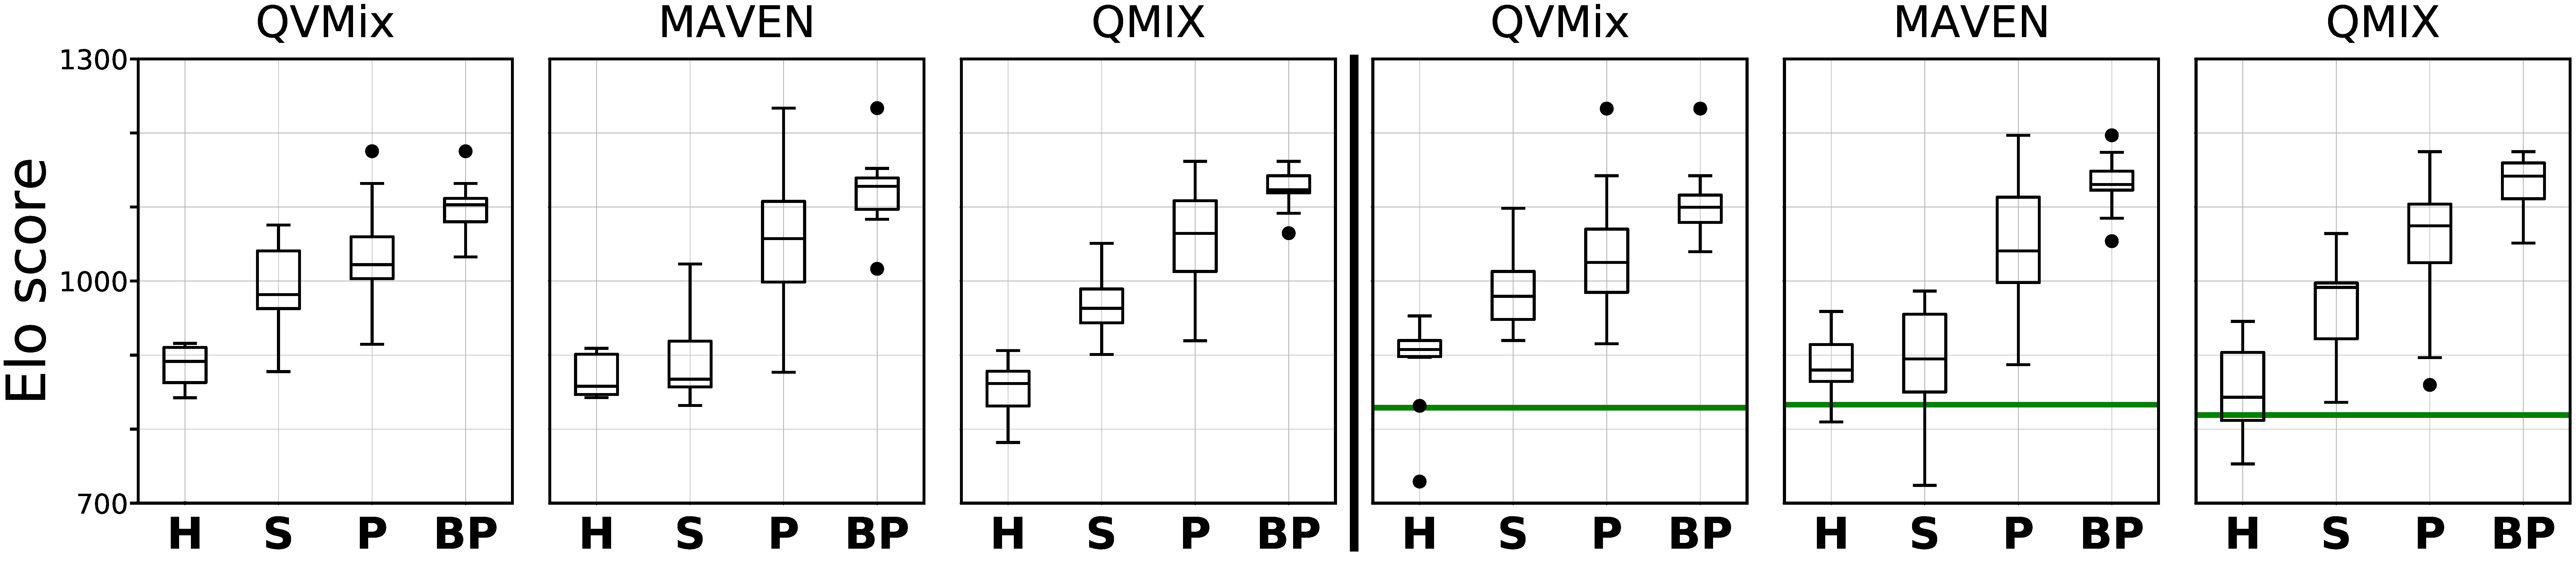
\includegraphics[width=\textwidth]{tex_thesis/figures/ch7/3m_tiny_six_qvmix_maven_qmix.pdf}
    \begin{subfigure}{.045\textwidth}
    \centering
    \caption*{}
    \end{subfigure}%
    \begin{subfigure}{.455\textwidth}
        \begin{subfigure}{.33\textwidth}
            \renewcommand\thesubfigure{\alph{subfigure}.1}
          \centering
          \caption{}
          \label{subfig:elo_no_h_methodQVMIX}
        \end{subfigure}%
        \begin{subfigure}{.33\textwidth}
        \addtocounter{subfigure}{-1}
            \renewcommand\thesubfigure{\alph{subfigure}.2}
          \centering
          \caption{}
          \label{subfig:elo_no_h_methodMAVEN}
        \end{subfigure}%
        \begin{subfigure}{.33\textwidth}
        \addtocounter{subfigure}{-1}
            \renewcommand\thesubfigure{\alph{subfigure}.3}
          \centering
          \caption{}
          \label{subfig:elo_no_h_methodQMIX}
        \end{subfigure}%
    \centering
    \addtocounter{subfigure}{-1}
    \caption{$3m$ map \textbf{without} heuristic.}
    \label{subfig:elo_no_h_3m}
    \end{subfigure}%
    \begin{subfigure}{.455\textwidth}
        \begin{subfigure}{.33\textwidth}
        \renewcommand\thesubfigure{\alph{subfigure}.1}
          \centering
          \caption{ }
          \label{subfig:elo_h_methodQVMIX}
        \end{subfigure}%
        \begin{subfigure}{.33\textwidth}
         \addtocounter{subfigure}{-1}
        \renewcommand\thesubfigure{\alph{subfigure}.2}
          \centering
          \caption{ }
          \label{subfig:elo_h_methodMAVEN}
        \end{subfigure}%
        \begin{subfigure}{.33\textwidth}
            \addtocounter{subfigure}{-1}
            \renewcommand\thesubfigure{\alph{subfigure}.3}
          \centering
          \caption{ }
          \label{subfig:elo_h_methodQMIX}
        \end{subfigure}%
    \centering
    \addtocounter{subfigure}{-1}
    \caption{$3m$ map \textbf{with} heuristic.}
     \label{subfig:elo_h_3m}
    \end{subfigure}%
    
    

    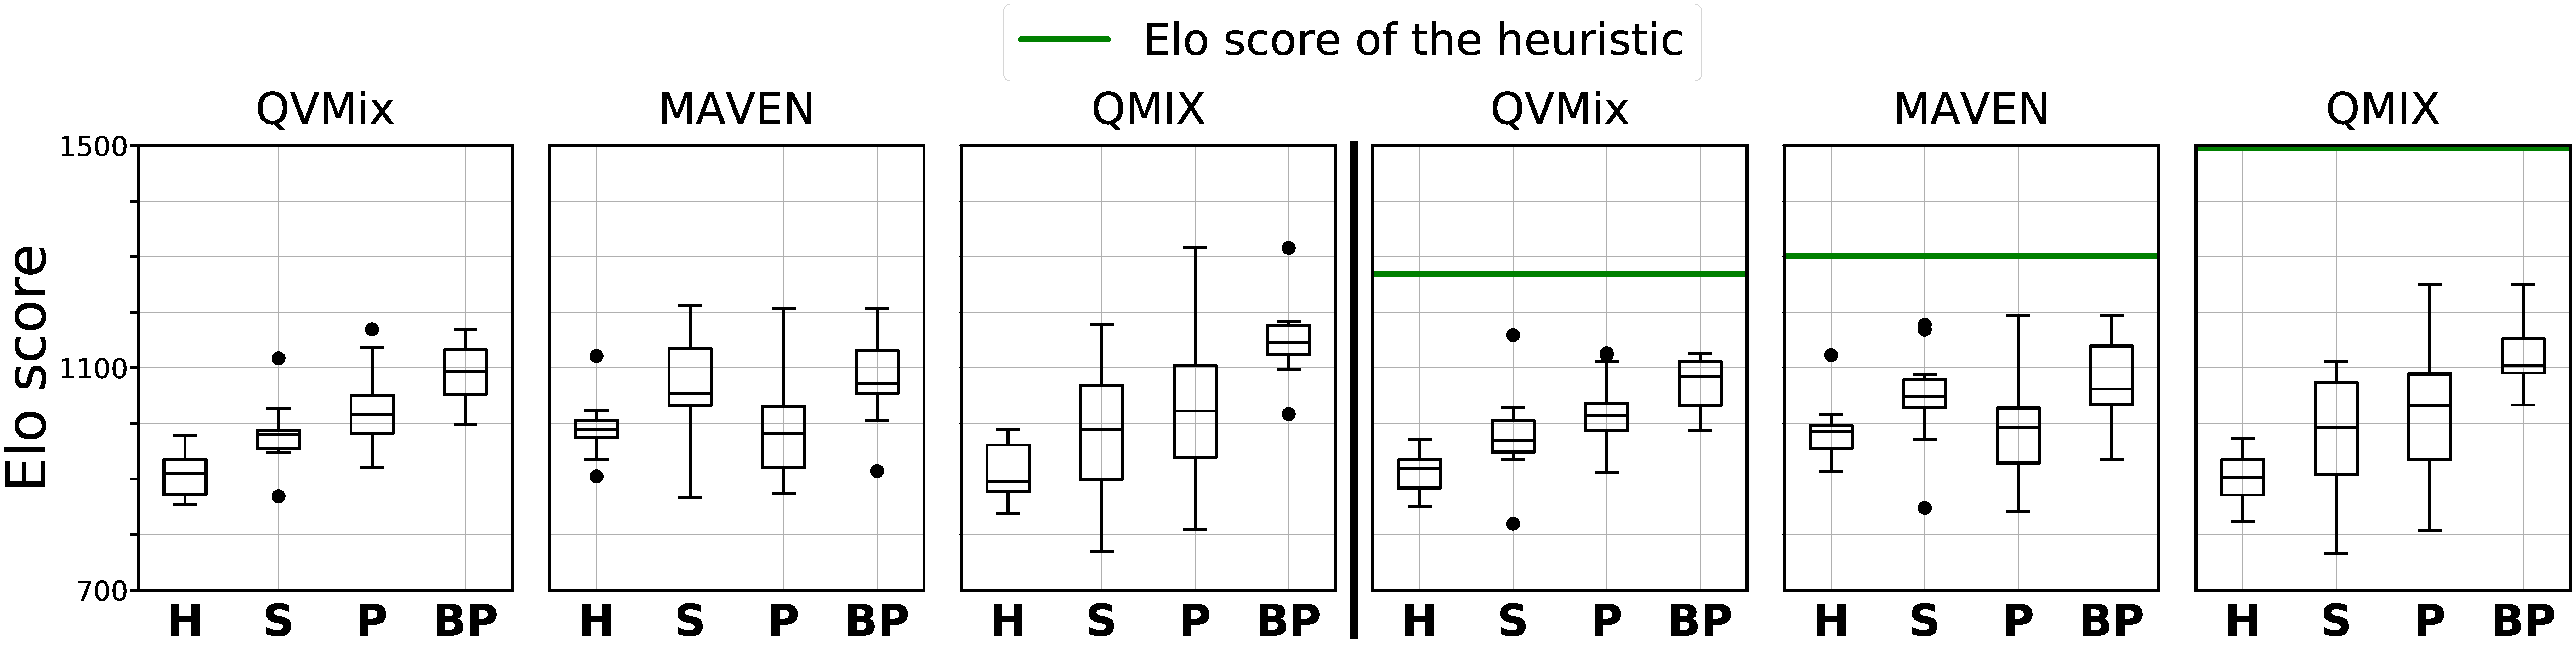
\includegraphics[width=\textwidth]{tex_thesis/figures/ch7/3s5z_tiny_six_qvmix_maven_qmix.pdf}
    \begin{subfigure}{.045\textwidth}
    \centering
    \caption*{}
    \end{subfigure}%
    \begin{subfigure}{.455\textwidth}
        \begin{subfigure}{.33\textwidth}
            \renewcommand\thesubfigure{\alph{subfigure}.1}
          \centering
          \caption{}
          \label{subfig:3s5z_elo_no_h_methodQVMIX}
        \end{subfigure}%
        \begin{subfigure}{.33\textwidth}
        \addtocounter{subfigure}{-1}
            \renewcommand\thesubfigure{\alph{subfigure}.2}
          \centering
          \caption{}
          \label{subfig:3s5z_elo_no_h_methodMAVEN}
        \end{subfigure}%
        \begin{subfigure}{.33\textwidth}
        \addtocounter{subfigure}{-1}
            \renewcommand\thesubfigure{\alph{subfigure}.3}
          \centering
          \caption{}
          \label{subfig:3s5z_elo_no_h_methodQMIX}
        \end{subfigure}%
    \centering
    \addtocounter{subfigure}{-1}
    \caption{$3s5z$ map \textbf{without} heuristic.}
     \label{subfig:elo_no_h_3s5z}
    \end{subfigure}%
    \begin{subfigure}{.455\textwidth}
        \begin{subfigure}{.33\textwidth}
        \renewcommand\thesubfigure{\alph{subfigure}.1}
          \centering
          \caption{ }
          \label{subfig:3s5z_elo_h_methodQVMIX}
        \end{subfigure}%
        \begin{subfigure}{.33\textwidth}
         \addtocounter{subfigure}{-1}
        \renewcommand\thesubfigure{\alph{subfigure}.2}
          \centering
          \caption{ }
          \label{subfig:3s5z_elo_h_methodMAVEN}
        \end{subfigure}%
        \begin{subfigure}{.33\textwidth}
            \addtocounter{subfigure}{-1}
            \renewcommand\thesubfigure{\alph{subfigure}.3}
          \centering
          \caption{ }
          \label{subfig:3s5z_elo_h_methodQMIX}
        \end{subfigure}%
    \centering
    \addtocounter{subfigure}{-1}
    \caption{$3s5z$ map \textbf{with} heuristic.}
     \label{subfig:elo_h_3s5z}
    \end{subfigure}%
    
    \caption{Elo score box plots of 12 test populations. 
    Half of the experiments were performed in the $3m$ map, shown at the top (\ref{subfig:elo_no_h_3m}, \ref{subfig:elo_h_3m}) and the other half in the $3s5z$ map, shown at the bottom (\ref{subfig:elo_no_h_3s5z}, \ref{subfig:elo_no_h_3s5z}). 
    In each test population, teams are trained with the same method, which is either QVMix (\ref{subfig:elo_no_h_methodQVMIX}, \ref{subfig:elo_h_methodQVMIX},\ref{subfig:3s5z_elo_no_h_methodQVMIX}, \ref{subfig:3s5z_elo_h_methodQVMIX}), MAVEN (\ref{subfig:elo_no_h_methodMAVEN}, \ref{subfig:elo_h_methodMAVEN},\ref{subfig:3s5z_elo_no_h_methodMAVEN}, \ref{subfig:3s5z_elo_h_methodMAVEN}) or QMIX (\ref{subfig:elo_no_h_methodQMIX}, \ref{subfig:elo_h_methodQMIX},\ref{subfig:3s5z_elo_no_h_methodQMIX}, \ref{subfig:3s5z_elo_h_methodQMIX}).
    In \ref{subfig:elo_h_3m} and \ref{subfig:elo_h_3s5z}, the heuristic is present in the test population and a green line represents its Elo score.
    Box plots represent the distribution of the ELO scores of the teams trained either against the heuristic (\textbf{H}), in self-play (\textbf{S}), within a population (\textbf{P}) or the best of each training population (\textbf{BP}).
    For most methods, teams trained within a population achieved the highest Elo scores.
    Box plots present the median, the first quantile ($Q1$) and the third quantile ($Q3$). The reach of whiskers is defined by $1.7*(Q3-Q1)$.
    }
    \label{fig:elo_method}

 
\end{figure*} 

We present the Elo scores of teams with box plots in Figure \ref{fig:elo_method} when the test population contains teams trained with the same method.
We first focus on performances when the heuristic is not in the test population (Fig. \ref{subfig:elo_no_h_3m}, \ref{subfig:elo_no_h_3s5z}).
The first observation is that the best teams are the ones trained within a population, except with MAVEN in $3s5z$ (Fig. \ref{subfig:3s5z_elo_no_h_methodMAVEN}) for which the differences between learning scenarios are smaller.
We discuss these differences later.
The second observation is that the population scenario has the highest variance.
To understand this, we also plot the box plots corresponding to the ten teams that achieved the highest Elo score of each training population, denoted by \textbf{BP}.
These box plots confirm that there is a difference between teams of the same training population and a selection must be performed to find the best one to optimise the performance of this learning scenario.
Training against the heuristic is the worst scenario, arguably because agents do not generalise to other strategies than the heuristic.
However, the heuristic is not in these test populations and its impact is the concern of later analysis.
The performance of teams trained in self-play lies between the two other learning scenarios.
While some achieve Elo scores close to those of the best teams in each training population, the scores of others are lower than the lowest scores of teams trained within the population.

The same experiment is performed by adding the heuristic in the three test populations, and corresponding box plots are presented in Figures \ref{subfig:elo_h_3m} and \ref{subfig:elo_h_3s5z}.
The heuristic scores are different depending on the map.
In the $3m$ map, most teams achieve a higher Elo score than the heuristic, whereas in $3s5z$, the heuristic dominates all teams.
Adding the heuristic slightly decreased Elo scores in the $3s5z$ map for all three learning scenarios.
The conclusion is straightforward and the heuristic is better than all teams.
However, one should note that the score ordering between the teams remained the same between Figure \ref{subfig:elo_no_h_3s5z} and \ref{subfig:elo_h_3s5z}.
In $3m$, one can see that the Elo score of teams trained against the heuristic (\textbf{H}) is higher in Fig. \ref{subfig:elo_h_3m} than the ones in Figure \ref{subfig:elo_no_h_3m}, as a direct consequence of the introduction into the test populations of a team against which they win.
When compared with the previous test populations (Fig. \ref{subfig:elo_no_h_3m}), teams trained with QVMix achieved higher Elo scores than without the heuristic in the test population (Fig. \ref{subfig:elo_h_methodQVMIX}).
In contrast, when trained with MAVEN and QMIX, they achieved lower Elo scores (Fig. \ref{subfig:elo_h_methodMAVEN}, \ref{subfig:elo_h_methodQMIX}).
In all cases, the higher values of box plots are not significantly different, but lower values are, meaning that some teams performed poorly against the heuristic.
The conclusion is that teams trained within a population remain the most successful in most of our experiments, no matter if the heuristic is the best or almost the worst team.

\begin{figure*}
    
\begin{subfigure}{\textwidth}
\centering
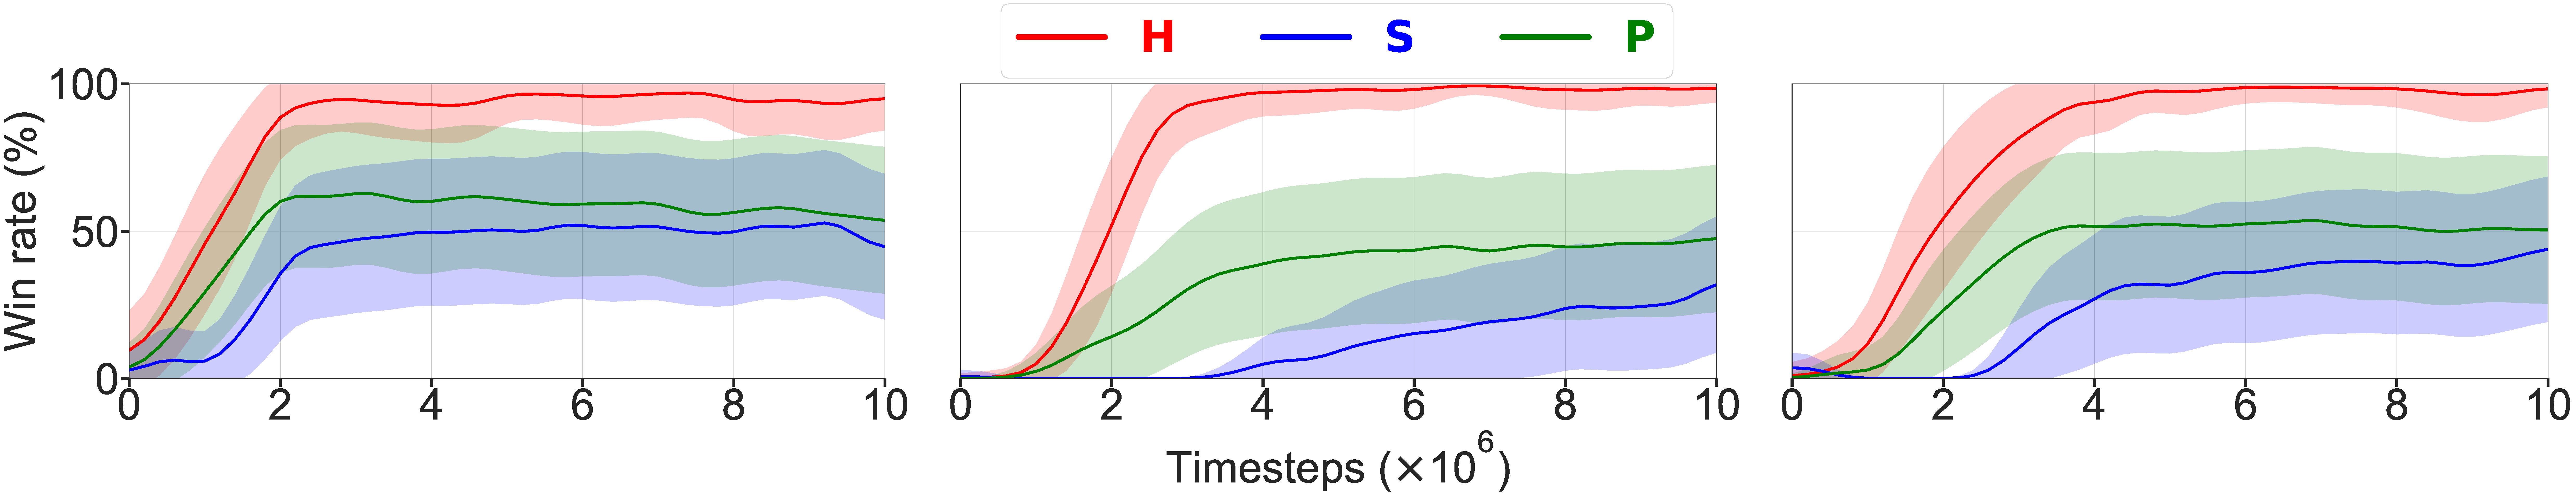
\includegraphics[width=.95\textwidth]{tex_thesis/figures/ch7/tiny_heuristic_plot_qvmixmavenqmix.pdf}
    \begin{subfigure}{.05\textwidth}
    \centering
    \caption*{}
    \end{subfigure}%
    \begin{subfigure}{.31\textwidth}
    \renewcommand\thesubfigure{\alph{subfigure}.1}
      \centering
      \caption{QVMix}
      \label{subfig:vs_h_methodQVMIX}
    \end{subfigure}%
    \begin{subfigure}{.31\textwidth}
    \addtocounter{subfigure}{-1}
    \renewcommand\thesubfigure{\alph{subfigure}.2}
      \centering
      \caption{MAVEN}
      \label{subfig:vs_h_methodMAVEN}
    \end{subfigure}%
    \begin{subfigure}{.31\textwidth}
    \addtocounter{subfigure}{-1}
    \renewcommand\thesubfigure{\alph{subfigure}.3}
      \centering
      \caption{QMIX}
      \label{subfig:vs_h_methodQMIX}
    \end{subfigure}
\addtocounter{subfigure}{-1}
\caption{Win rates achieved against the heuristic in the $3m$ map.}    
\label{subfig:3m_vs_h}
\end{subfigure}
\begin{subfigure}{\textwidth}
    \centering
    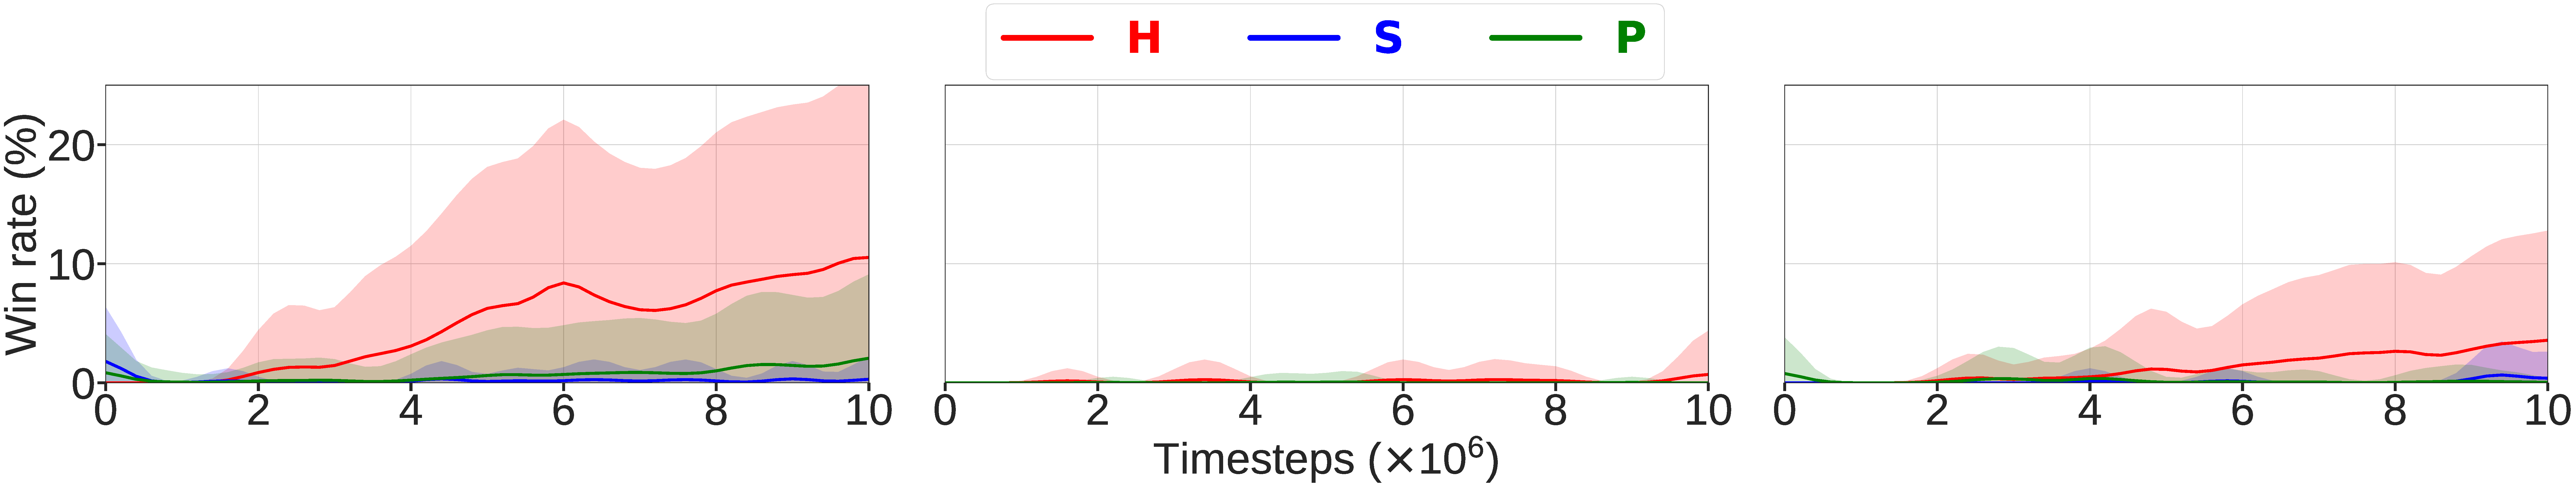
\includegraphics[width=.95\textwidth]{tex_thesis/figures/ch7/3s5z_tiny_heuristic_plot_qvmixmavenqmix.pdf}
    \begin{subfigure}{.05\textwidth}
    \centering
    \caption*{}
    \end{subfigure}%
    \begin{subfigure}{.31\textwidth}
    \renewcommand\thesubfigure{\alph{subfigure}.1}
      \centering
      \caption{QVMix}
      \label{subfig:3s5z_vs_h_methodQVMIX}
    \end{subfigure}%
    \begin{subfigure}{.31\textwidth}
    \addtocounter{subfigure}{-1}
    \renewcommand\thesubfigure{\alph{subfigure}.2}
      \centering
      \caption{MAVEN}
      \label{subfig:3s5z_vs_h_methodMAVEN}
    \end{subfigure}%
    \begin{subfigure}{.31\textwidth}
    \addtocounter{subfigure}{-1}
    \renewcommand\thesubfigure{\alph{subfigure}.3}
      \centering
      \caption{QMIX}
      \label{subfig:3s5z_vs_h_methodQMIX}
    \end{subfigure}
\addtocounter{subfigure}{-1}
\caption{Win rates achieved against the heuristic in the $3s5z$ map. Note the change in scale of the y-axis.}
\label{subfig:3s5z_vsh}
\end{subfigure}
\begin{subfigure}{\textwidth}
\centering
    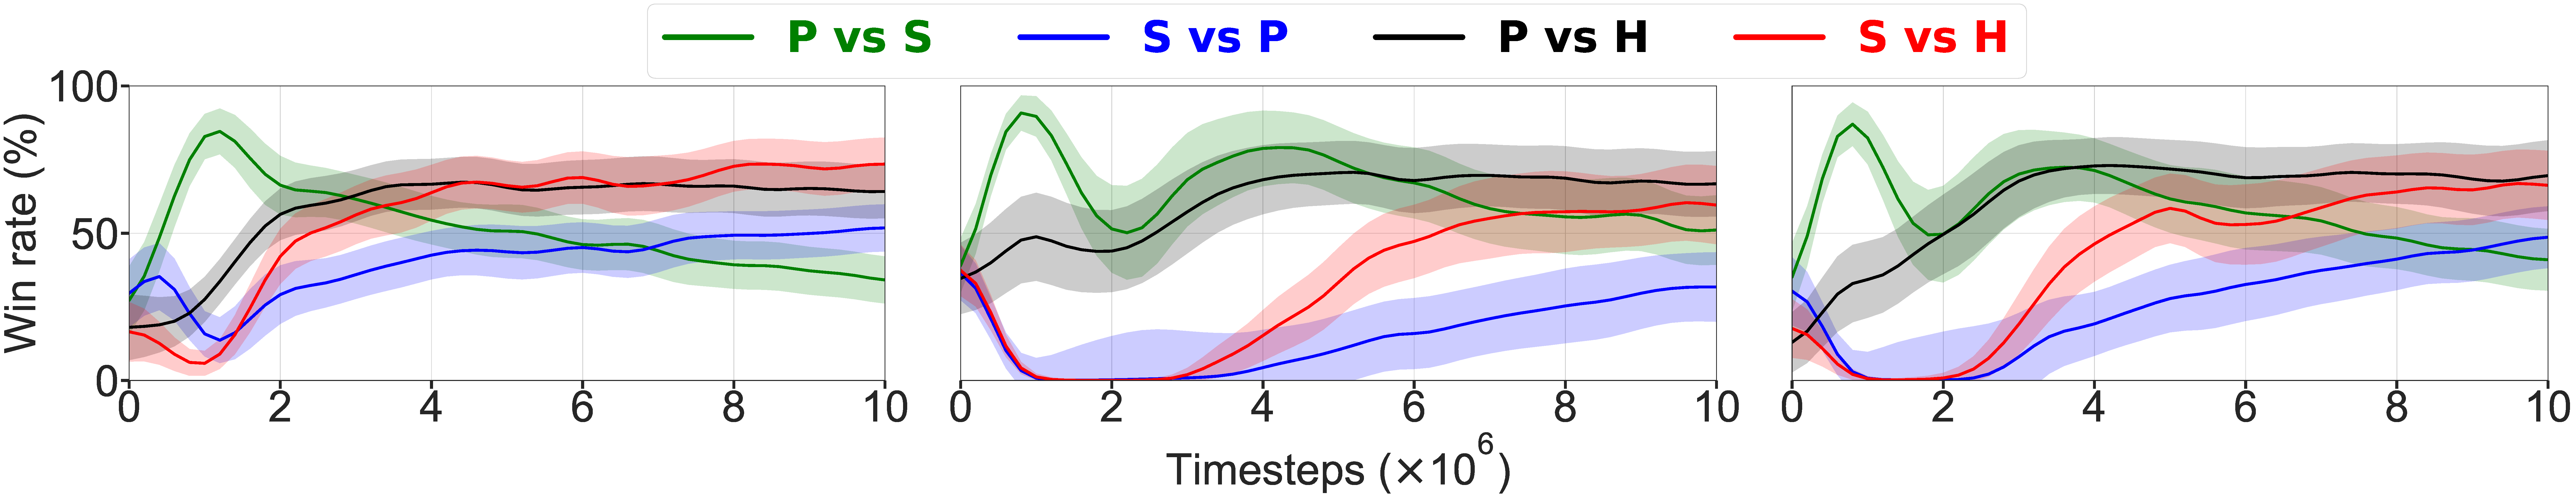
\includegraphics[width=.95\textwidth]{tex_thesis/figures/ch7/tiny_perf_self_popu.pdf}
    \begin{subfigure}{.05\textwidth}
    \centering
    \caption*{}
    \end{subfigure}%
    \begin{subfigure}{.31\textwidth}
    \renewcommand\thesubfigure{\alph{subfigure}.1}
      \centering
      \caption{QVMix}
      \label{subfig:duo_methodQVMIX}
    \end{subfigure}%
    \begin{subfigure}{.31\textwidth}
    \addtocounter{subfigure}{-1}
    \renewcommand\thesubfigure{\alph{subfigure}.2}
      \centering
      \caption{MAVEN}
      \label{subfig:duo_methodMAVEN}
    \end{subfigure}%
    \begin{subfigure}{.31\textwidth}
    \addtocounter{subfigure}{-1}
    \renewcommand\thesubfigure{\alph{subfigure}.3}
      \centering
      \caption{QMIX}
      \label{subfig:duo_methodQMIX}
    \end{subfigure}
\addtocounter{subfigure}{-1}
\caption{Win rates achieved by teams trained in the $3m$ map against themselves.}
\label{subfig:3m_duo}
\end{subfigure}
\begin{subfigure}{\textwidth}
\centering
    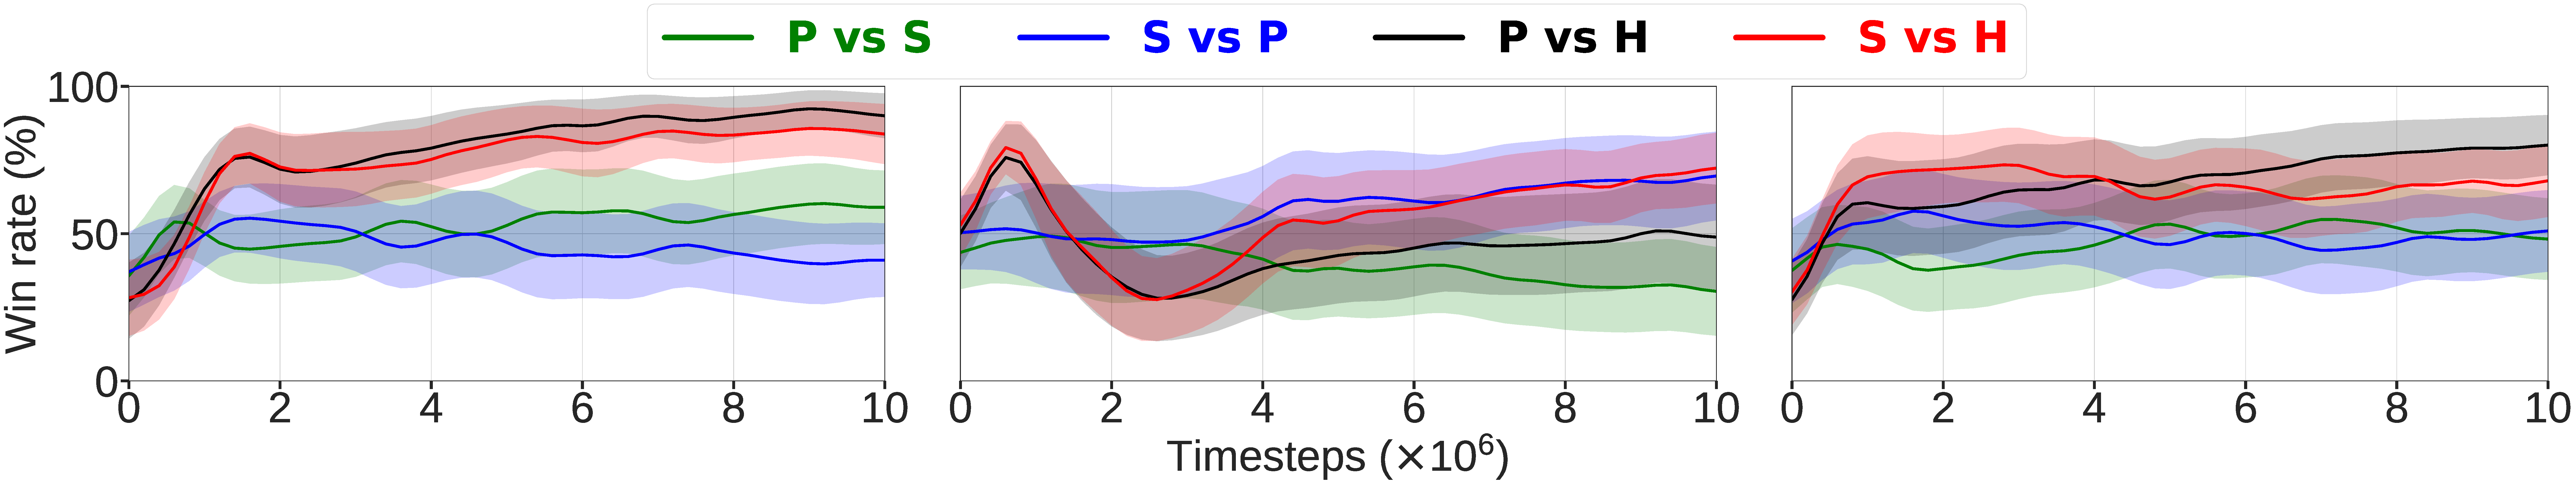
\includegraphics[width=.95\textwidth]{tex_thesis/figures/ch7/3s5z_tiny_perf_self_popu.pdf}
    \begin{subfigure}{.05\textwidth}
    \centering
    \caption*{}
    \end{subfigure}%
    \begin{subfigure}{.31\textwidth}
    \renewcommand\thesubfigure{\alph{subfigure}.1}
      \centering
      \caption{QVMix}
      \label{subfig:3s5z_duo_methodQVMIX}
    \end{subfigure}%
    \begin{subfigure}{.31\textwidth}
    \addtocounter{subfigure}{-1}
    \renewcommand\thesubfigure{\alph{subfigure}.2}
      \centering
      \caption{MAVEN}
      \label{subfig:3s5z_duo_methodMAVEN}
    \end{subfigure}%
    \begin{subfigure}{.31\textwidth}
    \addtocounter{subfigure}{-1}
    \renewcommand\thesubfigure{\alph{subfigure}.3}
      \centering
      \caption{QMIX}
      \label{subfig:3s5z_duo_methodQMIX}
    \end{subfigure}
\addtocounter{subfigure}{-1}
\caption{Win rates achieved by teams trained in the $3s5z$ map against themselves.}
\label{subfig:3s5z_duo}
\end{subfigure}

\caption{
Means of win rate achieved along training time steps by confronting teams trained with the same method against the heuristic or against other teams trained with a different learning scenario.
Teams are trained either with QVMix, MAVEN, or QMIX.
Tests were performed in the $3m$ map, shown at the top, and in the $3s5z$ maps, shown at the bottom. 
Win rates against the heuristic are presented in red, blue and green for teams trained against the heuristic, in self-play and within a population, respectively.
Win rates of teams trained within a population against teams trained in self-play are presented in green and against teams trained against the heuristic in black.
Win rates of teams trained in self-play against teams trained within a population are presented in blue and against teams trained against the heuristic in red.
The error band is half the standard deviation.
} 
\label{fig:heuristic_plot}
\end{figure*}

In Figure \ref{subfig:3m_vs_h}, we present the evolution of win rates against the heuristic along training timesteps by each team in the $3m$ map.
For all methods, teams trained against the heuristic are the best against it on average.
This explains why their Elo scores improve when the heuristic is included in the test population.
This is also the case for QVMix teams trained in self-play and within a population that performed better and learned faster than teams trained with MAVEN and QMIX with these two learning scenarios.
However, in the $3s5z$ map, it can be seen in Figure \ref{subfig:3s5z_vsh} that the win rates against the heuristic are very low, not to say equal to zero.
Only the win rates of teams trained against the heuristic, especially with QVMix and QMIX, increase at the end of the training but with a high variance in comparison to the $3m$ map (Fig. \ref{subfig:3m_vs_h}).
For QVMix, the win rates of teams trained with a population also increase at the end of the training phase.
The time we have budgeted for training in the $3s5z$ map may be insufficient to achieve a high win rate.
However, we find this beneficial because it shows that, even when the heuristic is better than all teams, training against it, with the same training timesteps allowance, is not the best learning scenario when teams have to be good against several strategies.
This also shows that our heuristic is harder to defeat with respect to the results of \citep{Rashid2018,Mahajan2019MAVEN:Exploration,leroy2020qvmix} where better results are observed in these maps with the former SMAC heuristic.

In the $3m$ map, the standard deviation of green and blue win rates, representing population and self-play learning scenarios, respectively, is high.
This confirms the results of Elo score box plots that there are performance gaps between teams trained within the same learning scenario.
Observations also suggest that if trained for longer, teams trained in self-play would achieve the same win rates as teams trained within a population, suggesting a difference in training sample efficiency.
As teams first need to learn to cross the map to meet opponents and fight them, this difference is maybe because training within a population against several strategies increases the probability of creating episodes where two opposing agents meet and fight at the beginning of training.

Figures \ref{subfig:3m_duo} and \ref{subfig:3s5z_duo} show win rates from the confrontations between trained teams.
The draw rates can be obtained by subtracting from $1$ the sum of these two curves.
This confirms the previous results with box plots that training against the heuristic is the worst scenario, as an average win rate above $60\%$ is achieved against them, as shown in the black and red curves.
Green and blue curves enable one to analyse self-play against population-learning scenarios.
At the beginning of the training phase, teams trained within a population are better than self-play in the $3m$ map.
This high win rate decreases with training in favour of the win rate of teams trained in self-play for QVMix and QMIX until it becomes higher than the latter.
Again, this suggests a difference in training sample efficiency.
Moreover, although the training sample efficiency is lower for teams trained in self-play, the number of environment timesteps required to train them is five times lower in our setting.
However, it is on average that the self-play teams become better.
In the $3s5z$ map, this overlap phenomenon does not occur, and the average win rates fluctuate around $50\%$ with the green curves remaining just above the blue ones at the end.
The proximity of performances between teams trained in self-play and within a population is arguably due to the environment and the $3m$ map, which does not offer the possibility of winning with very different strategies.
As the $3s5z$ map appears to be more complex, with the lack of performances against the heuristic as evidence, teams trained within a population remain better on average.

\begin{figure*}[ht]
\begin{subfigure}{\textwidth}
\centering
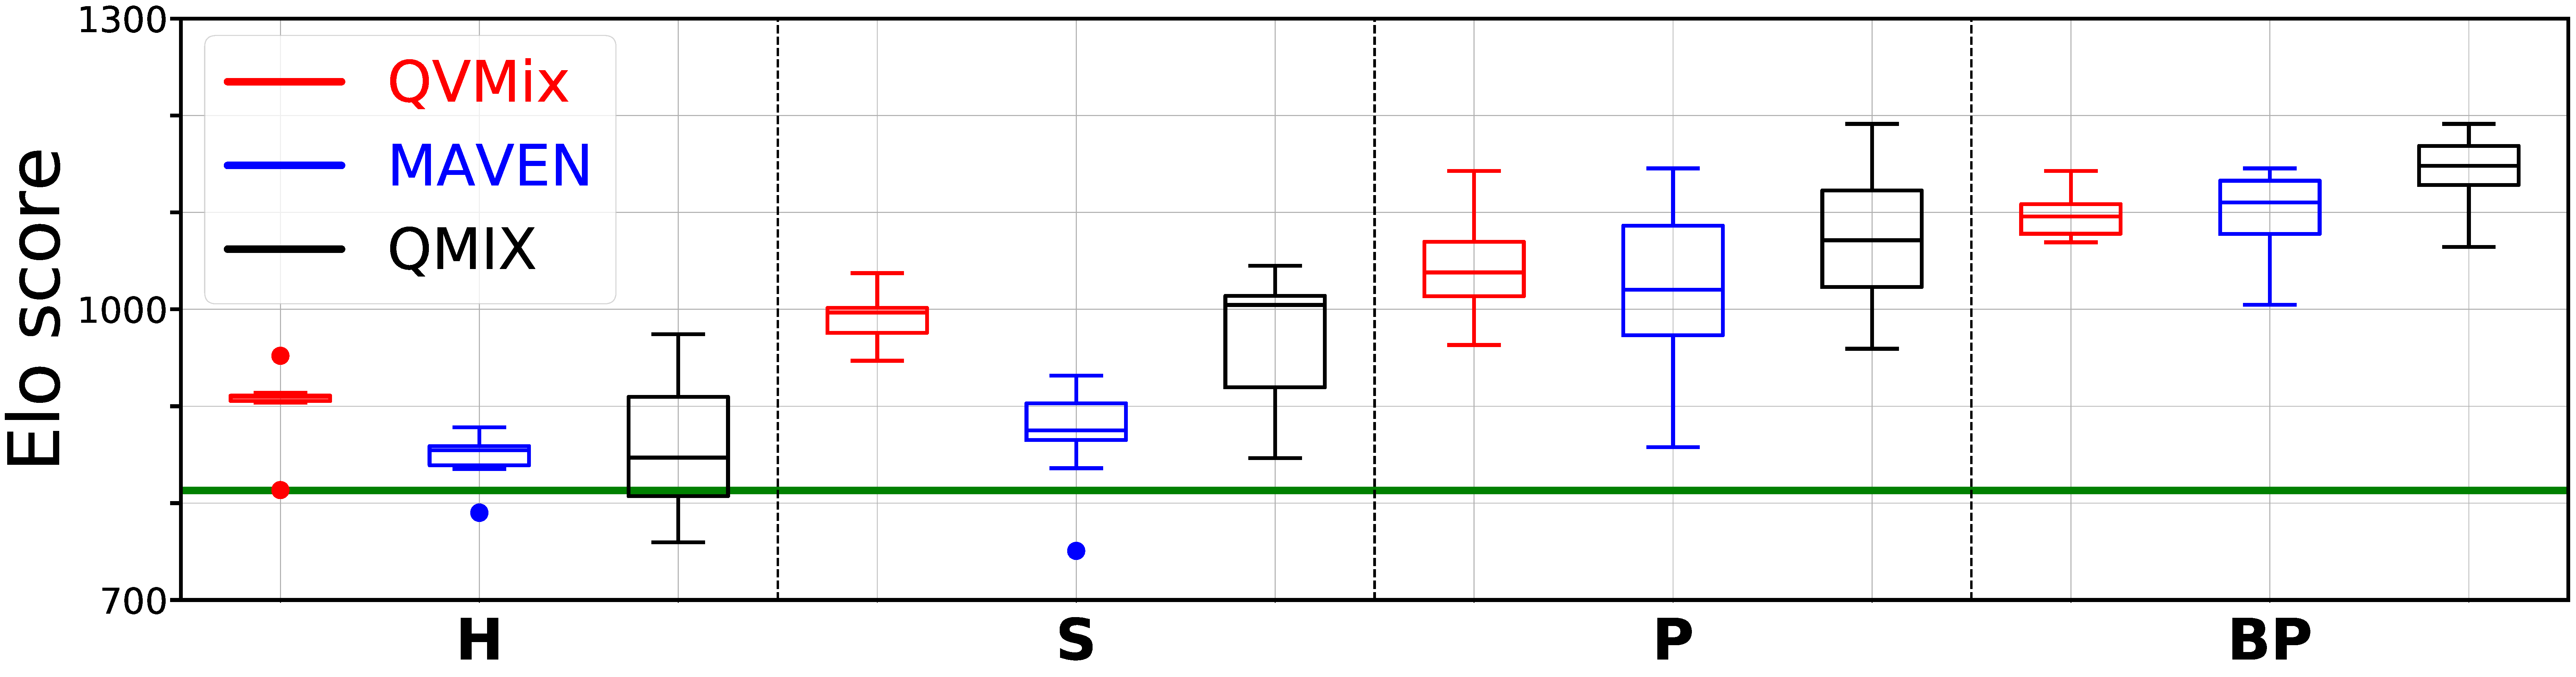
\includegraphics[width=.95\textwidth]{tex_thesis/figures/ch7/3m_tiny_all_h_clean.pdf}
\caption{$3m$ map \textbf{with} the heuristic.}
\label{subfig:3m_all_h}
\end{subfigure}
\begin{subfigure}{\textwidth}
\centering
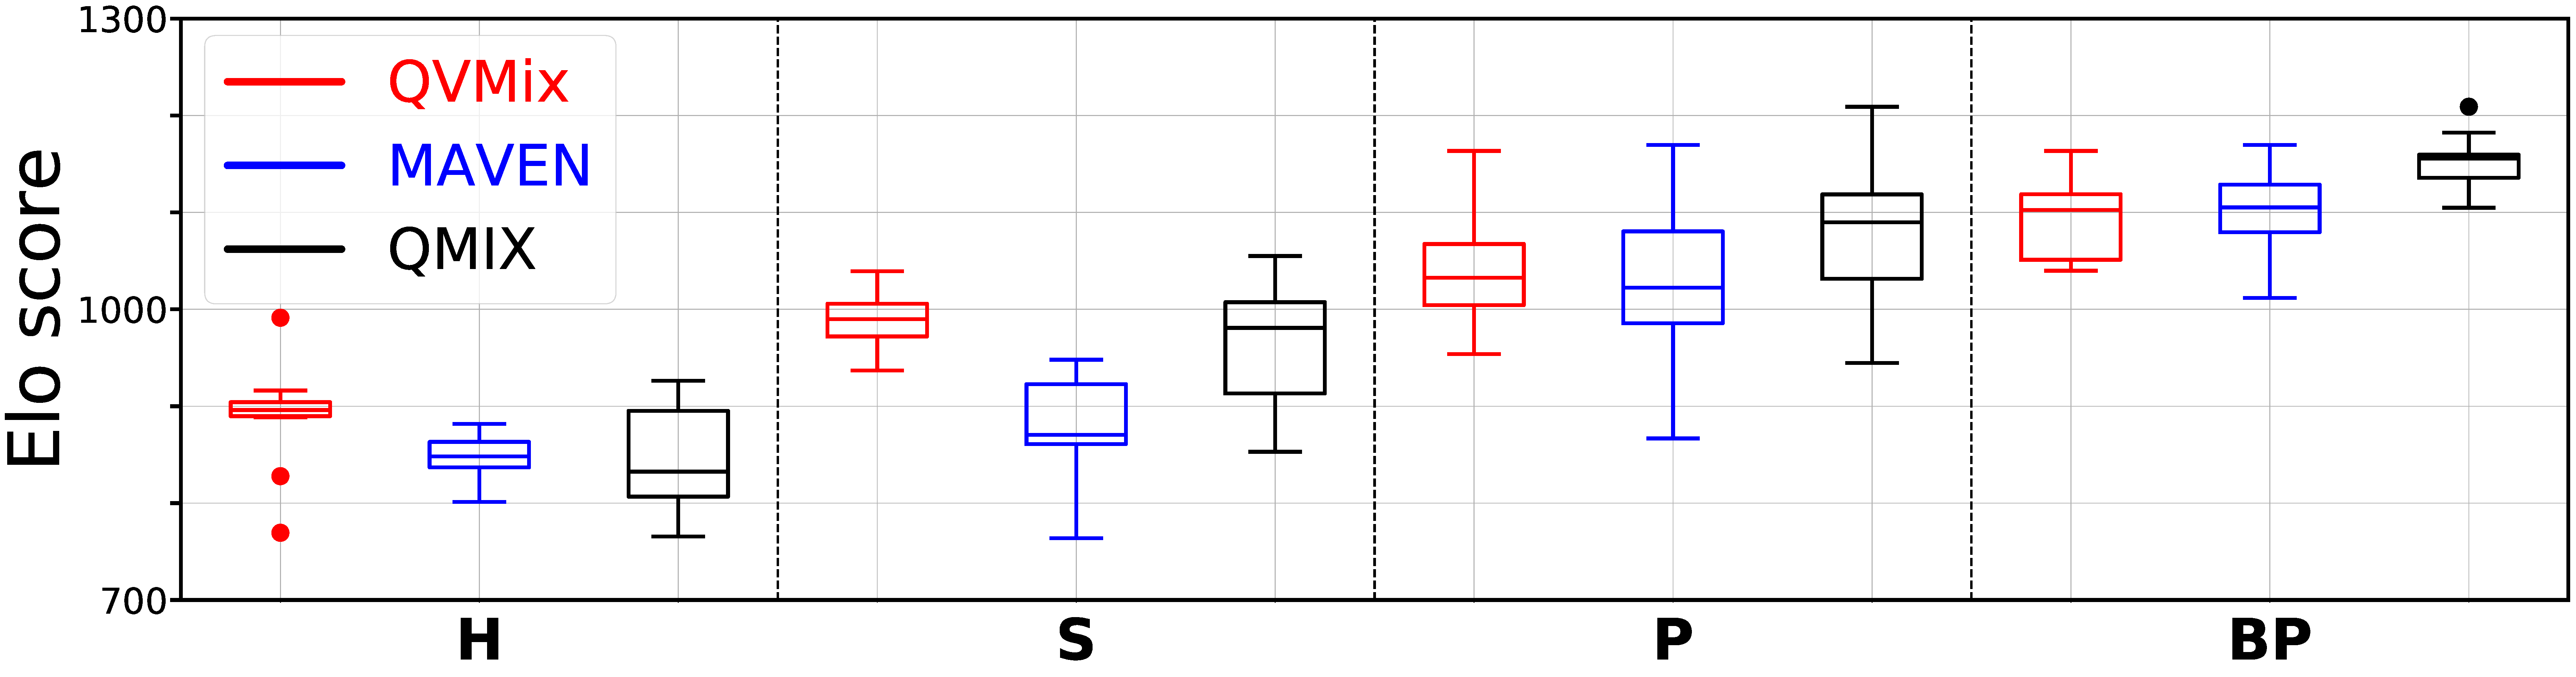
\includegraphics[width=\textwidth]{tex_thesis/figures/ch7/3m_tiny_all_no_h_clean.pdf}
\caption{$3m$ map \textbf{without} the heuristic.}
\label{subfig:3m_all_no_h}
\end{subfigure}
\begin{subfigure}{\textwidth}
\centering
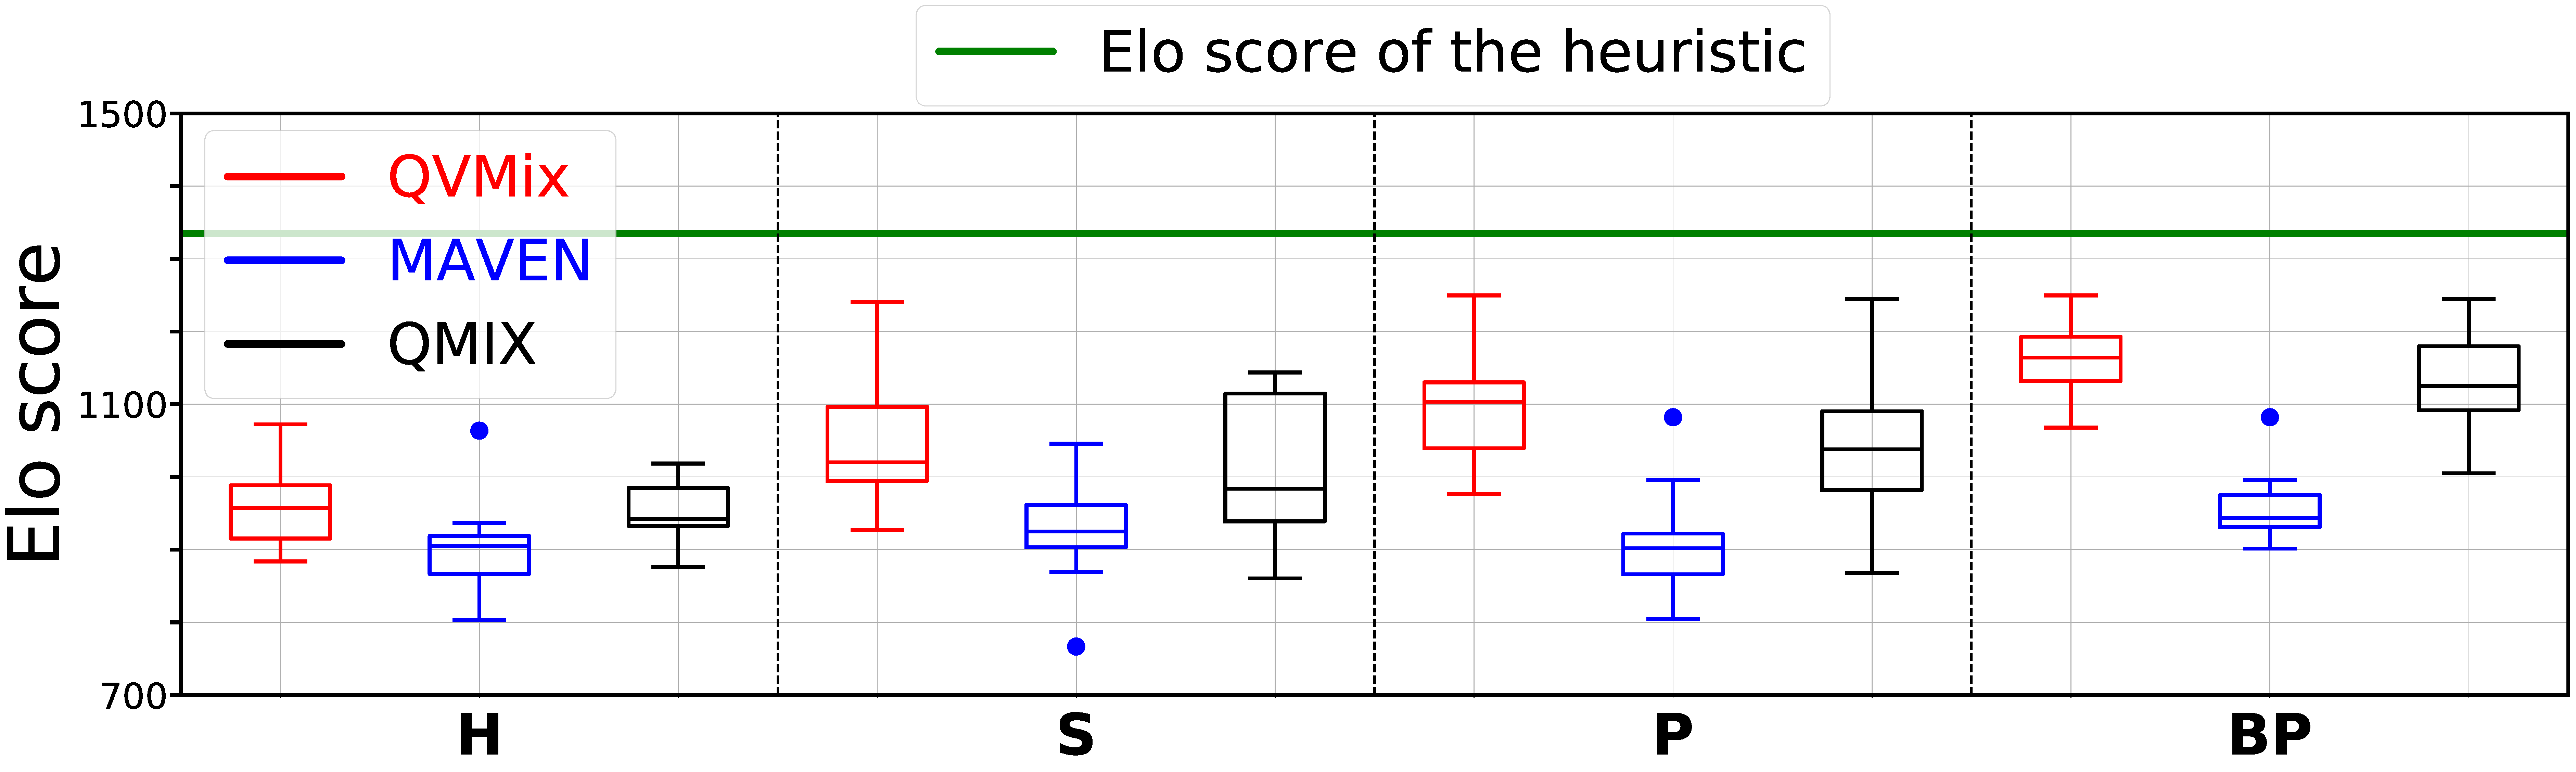
\includegraphics[width=.95\textwidth]{tex_thesis/figures/ch7/3s5z_tiny_all_h_clean.pdf}
\caption{$3s5z$ map \textbf{with} the heuristic.}
\label{subfig:3s5z_all_h}
\end{subfigure}
\begin{subfigure}{\textwidth}
\centering
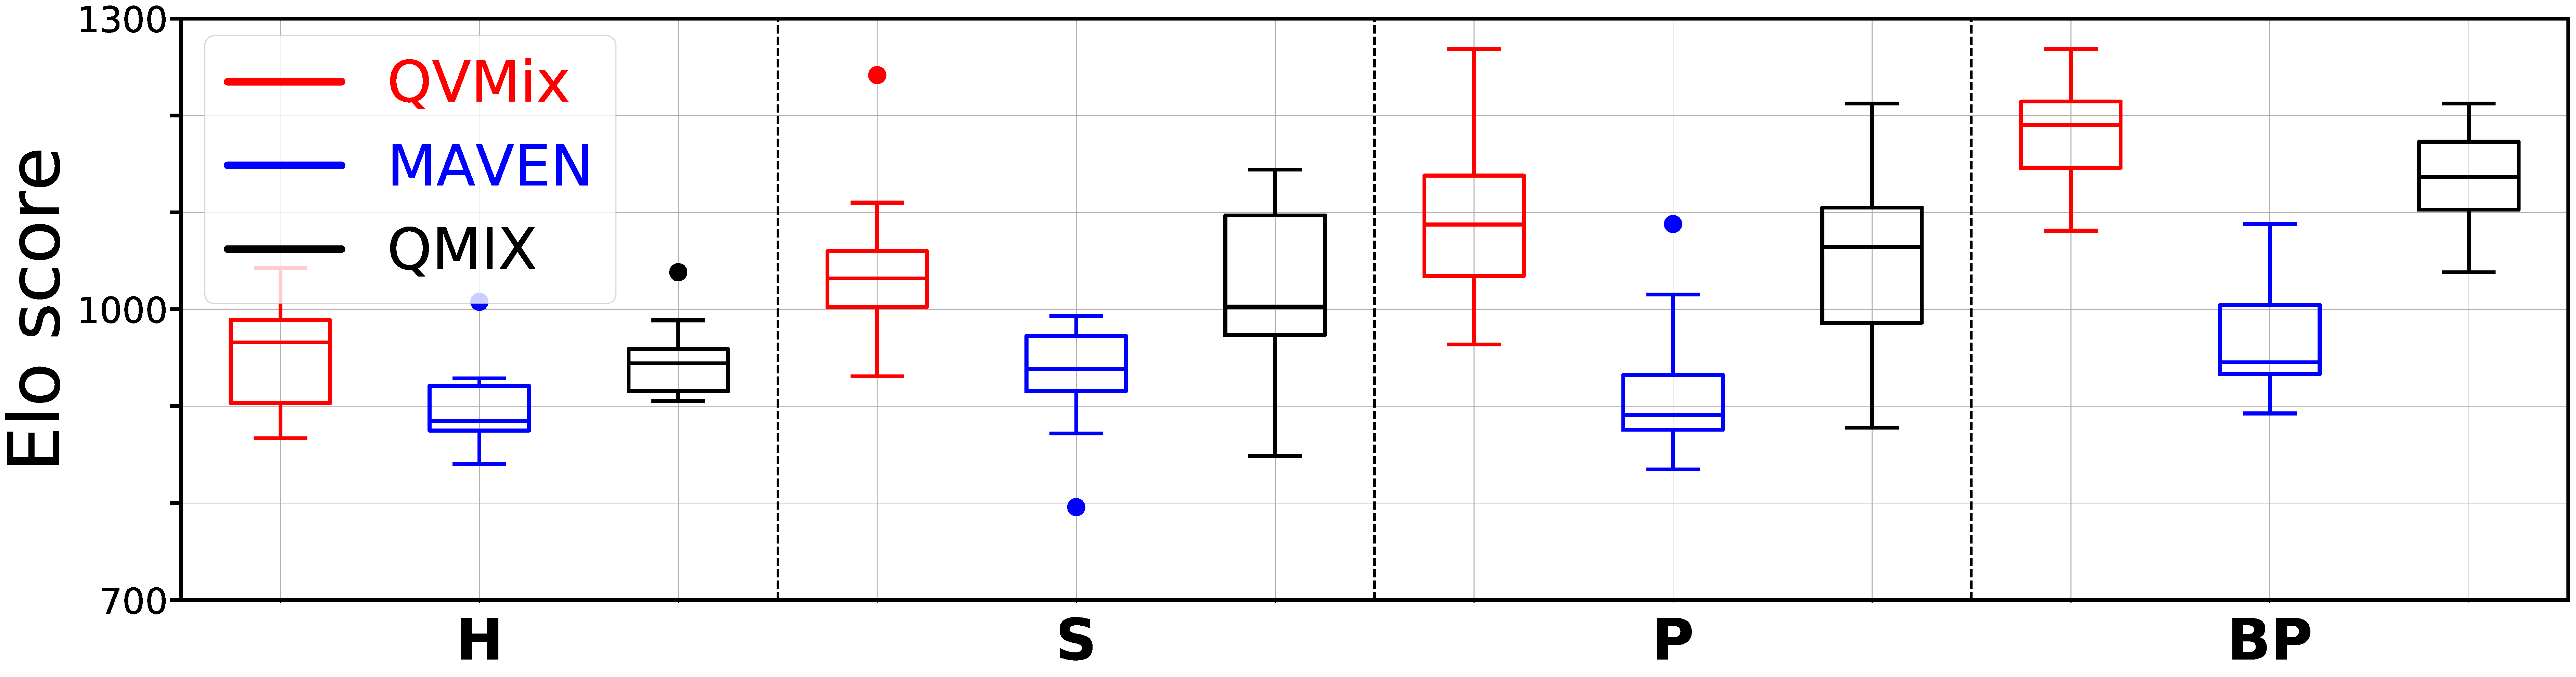
\includegraphics[width=\textwidth]{tex_thesis/figures/ch7/3s5z_tiny_all_no_h_clean.pdf}
\caption{$3s5z$ map \textbf{without} the heuristic.}
\label{subfig:3s5z_all_no_h}
\end{subfigure}
\caption{
Elo score box plots of four test populations, in $3m$ at the top and $3s5z$ at the bottom, composed of teams trained using three methods and three learning scenarios, with and without the heuristic.
The training method is either QVMix (red), MAVEN (blue) or QMIX (black).
Box plots represent the distribution of the ELO scores of teams trained either against the heuristic (\textbf{H}), in self-play (\textbf{S}), within a population (\textbf{P}) or the best of each population (\textbf{BP}).
Box plots present the median, the first quantile ($Q1$) and the third quantile ($Q3$). The reach of whiskers is defined by $1.7*(Q3-Q1)$.
}
\label{fig:all}
\end{figure*}

On average, the results of the teams trained within a population with MAVEN in the $3s5z$ map differ from the other experiments. 
Some results are slightly worse when compared to those of the other experiments.
The reason for this is unsure, as we executed the experiments several times, but this does not affect the conclusions of our experiments that remain clear.
Finally, it would be necessary to repeat these experiments more times or to analyse the agents' behaviour in depth to find the problem, which is beyond the scope of the study. 

In Figure \ref{fig:all}, we present the box plots of Elo scores obtained when grouping all trained teams in a single test population for both maps, with and without the heuristic.
The learning scenario ranking remains the same as in other experiments.
In the $3m$ map, QMIX achieves the highest Elo scores, while the lowest MAVEN Elo scores are worse than the ones of QMIX and QVMix when teams are trained in self-play or within a population.
QVMix produces results with a lower variance than QMIX.
In the $3s5z$ map, QVMix achieves the highest Elo scores, and MAVEN achieves the lowest ones.
The same experiment without the heuristic led to the same conclusion.
Despite its exploration mechanism, MAVEN cannot outperform QMIX and QVMix.
This is also the case in \citep{Mahajan2019MAVEN:Exploration} and \citep{leroy2020qvmix}, where they show that MAVEN outperforms QMIX but not QVMix in more complex Dec-POMDP environments.


\section{Discussion and future work} \label{sec:ch7_conclu}
This study evaluated learning scenarios to train teams to face multiple strategies in a symmetric two-team Markov game.
Teams are trained with three value-based CTDE methods, QMIX, MAVEN, and QVMix, and with three learning scenarios differentiated by the variety of strategies they will encounter during their training.
Specifically, they are trained by playing against a stationary strategy, against themselves, or within a population of teams trained using the same method.
To perform our experiments, we modified the cooperative environment SMAC to allow teams to compete and train simultaneously and trained teams in two different SMAC environments.
The Elo rating system evaluates these nine types of trained teams at the end of their training.
Different groups are formed to identify the best learning scenario and the best learning scenario/training method pair.
We also analysed the win rates of several matchups during training to support the results provided by the Elo scores.
Our results showed that the best learning scenario is to train teams within a population of learning teams when each team plays the same number of timesteps for training purposes.
We reached this conclusion irrespective of whether or not the stationary strategy was better than all trained teams.
Finally, a selection procedure is required because teams from the same training population do not perform equally.

This work is one of the first investigations of two-team competition with CTDE methods, and we hereafter suggest several future research directions.
First, we suggest performing the same experiments on more complex environments and tackling the challenges of asymmetric settings.
In this paper, we selected value-based methods because of their performances in SMAC \citep{samvelyan2019starcraft} at the time of our experiments.
Recent CTDE methods overcome these performances and may lead to interesting new results.
Typically, stochastic policies trained with policy-based methods might provide better results in our setting.
Another research direction would be to study how diversity in the training population impacts performance. 
Diversity could be increased by adding the heuristic in the population, confronting agents against older learned policies, varying the size of the population or training teams with different methods in the same population.
In addition, as described in Chapter \ref{ch:competition}, methods that compute the best responses or model the opponent would be interesting to test in such an environment.
We also propose performing behavioural and policy analyses to better understand why some teams achieve a better Elo score and how strategies differ in a single training population.